% Copyright 2004 by Till Tantau <tantau@users.sourceforge.net>.
%
% In principle, this file can be redistributed and/or modified under
% the terms of the GNU Public License, version 2.
%
% However, this file is supposed to be a template to be modified
% for your own needs. For this reason, if you use this file as a
% template and not specifically distribute it as part of a another
% package/program, I grant the extra permission to freely copy and
% modify this file as you see fit and even to delete this copyright
% notice. 

\documentclass{beamer}
\usepackage{graphicx}

% There are many different themes available for Beamer. A comprehensive
% list with examples is given here:
% http://deic.uab.es/~iblanes/beamer_gallery/index_by_theme.html
% You can uncomment the themes below if you would like to use a different
% one:
%\usetheme{AnnArbor}
%\usetheme{Antibes}
%\usetheme{Bergen}
%\usetheme{Berkeley}
%\usetheme{Berlin}
\usetheme{Boadilla}
%\usetheme{boxes}
%\usetheme{CambridgeUS}
%\usetheme{Copenhagen}
%\usetheme{Darmstadt}
%\usetheme{default}
%\usetheme{Frankfurt}
%\usetheme{Goettingen}
%\usetheme{Hannover}
%\usetheme{Ilmenau}
%\usetheme{JuanLesPins}
%\usetheme{Luebeck}
%\usetheme{Madrid}
%\usetheme{Malmoe}
%\usetheme{Marburg}
%\usetheme{Montpellier}
%\usetheme{PaloAlto}
%\usetheme{Pittsburgh}
%\usetheme{Rochester}
%\usetheme{Singapore}
%\usetheme{Szeged}
%\usetheme{Warsaw}

\usepackage[utf8]{inputenc}
\usepackage{outlines}

\graphicspath{{./img/}}

\title{Colectarea și analiza datelor din procesul de tipărire folosind tehnologii distribuite}
\subtitle{Prezentare sintetică}

\titlegraphic{ 
\includegraphics[width=2cm]{upt_logo.png} }

\author{Andrei Buruntia}

\date{20/06/2018}

\subject{Theoretical Computer Science}
\AtBeginSubsection[]
{
  \begin{frame}<beamer>{Outline}
    \tableofcontents[currentsection,currentsubsection]
  \end{frame}
}

% Let's get started
\begin{document}

\begin{frame}
  \titlepage
\end{frame}

\begin{frame}{Cuprins}
  \tableofcontents
  % You might wish to add the option [pausesections]
\end{frame}

% Section and subsections will appear in the presentation overview
% and table of contents.
\section{Motivație}
\begin{frame}{Motivație}	
	\begin{center}
		
\includegraphics[width=50mm]{oce_logo.png}
	\end{center}
\end{frame}
\section{Problema}
\begin{frame}{Problema}
	\begin{itemize}[<+->]
	\item extragerea datelor din procesul de tipărire
	\item analiza facilă a informațiilor extrase
	\item compunerea unor grafice care să releve trenduri sau tipare relevante
	\end{itemize}
\end{frame}
\section{Implementare}
\subsection{Tehnologii folosite}
\begin{frame}{Implementare}{Tehnologii folosite}
	\begin{outline}
 	\1 `familia' Unix
 	\1 CUPS
 	\1 ELK stack
 		\2 Beat
 		\2 Elasticsearch
 		\2 Kibana
	\end{outline}
\end{frame}
\subsection{Arhitectură}
\begin{frame}{Implementare}{Arhitectură}
	\begin{center}
		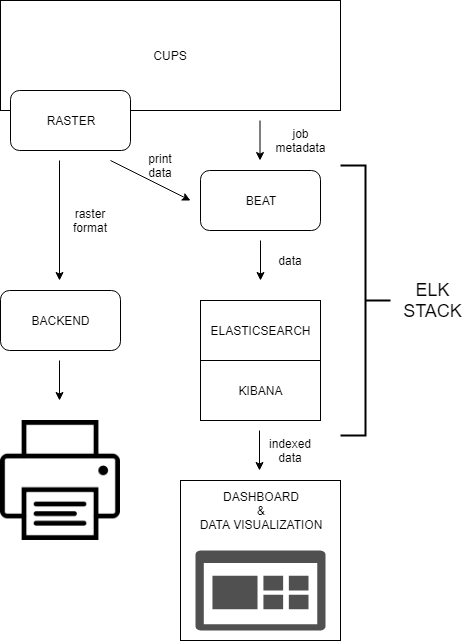
\includegraphics[width=50mm]{cups.png}
	\end{center}
\end{frame}
\begin{frame}{Introducere}{Arhitectură}
	\begin{center}
		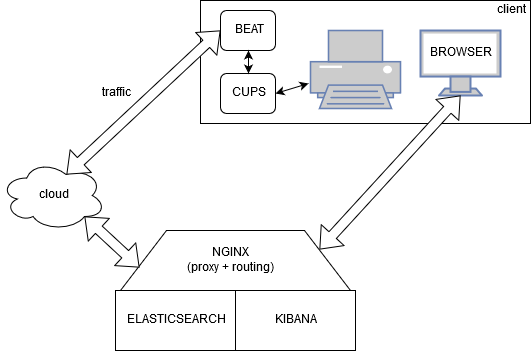
\includegraphics[width=50mm]{cups-cloud.png}
	\end{center}
\end{frame}
\subsection{Interconectarea modulelor}
\begin{frame}{Implementare}{Interconectarea modulelor}
	\begin{itemize}[<+->]
	\item CUPS - Beat: named pipe/FIFO
	\item Beat - Elasticsearch - Kibana: protocol intern al stivei ELK peste HTTP
	\end{itemize}
\end{frame}


% Placing a * after \section means it will not show in the
% outline or table of contents.
\section*{Rezumat}

\begin{frame}{Rezumat}
  \begin{itemize}[<+->]
  \item
    Proiectul a presupus realizarea unui sistem care să \alert{preia date din CUPS} intr-un mod \alert{non-invaziv} și găsirea unei modalități de a prelucra datele spre a fi afișate utilizatorului sub forma unor \alert{grafice ușor de înțeles}.
    \item
    Folosirea tehnologiilor \alert{open-source} a păstrat complexitatea proiectului la un nivel relativ redus.
    \item
    Am remarcat \alert{robustețea stivei ELK și a sistemului de tipărire CUPS}. 
  \end{itemize}
  
\end{frame}

\end{document}

